

% Early Allies, Late Divergence
% From Allies to Antagonists: The Divergent Trajectory of Gradient Evolution
% Aligned Effort, Diminishing Impact
% 

\begin{wrapfigure}[11]{r}{0.47\columnwidth}
    \vspace{-1.2em}
    \centering
    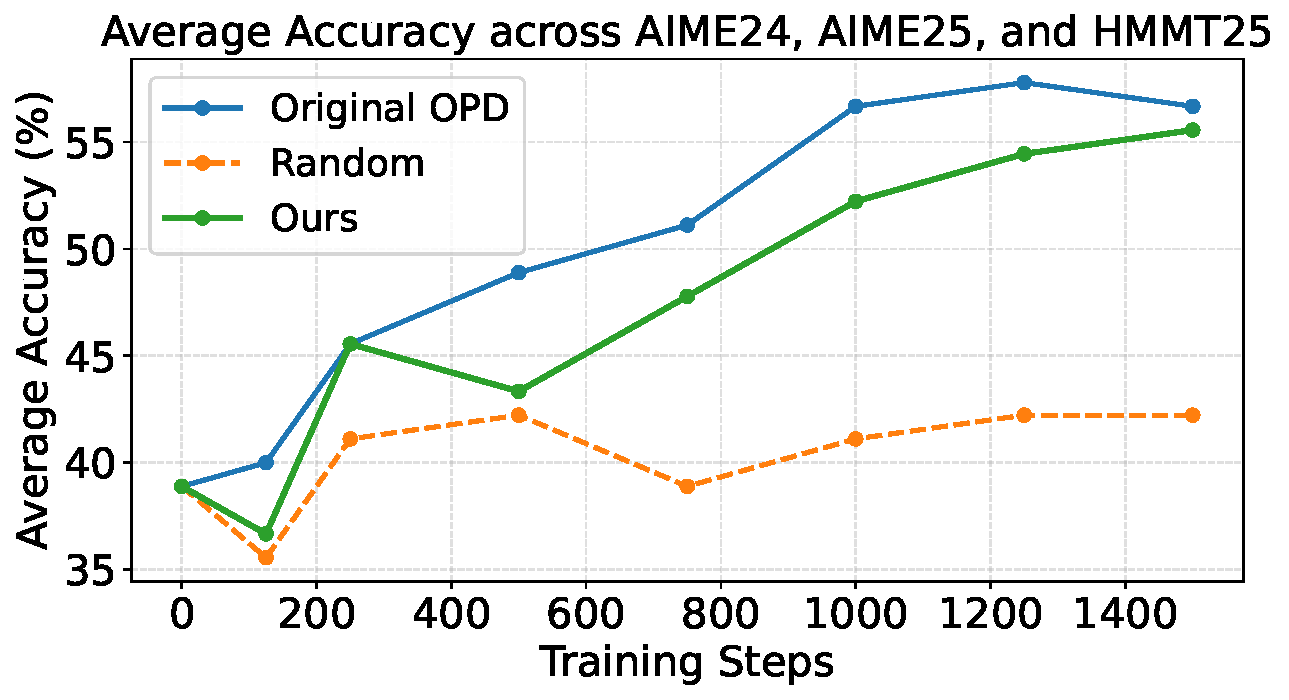
\includegraphics[width=0.45\columnwidth]{Figures/opd_random_vs_ours_avg.pdf}
    \vspace{-0.8em}
    \caption{
    Average accuracy across AIME24, AIME25, and HMMT25 during OPD training. Each 200 training steps correspond to 8,000 prompts, with 4 rollouts per prompt.
    }
    \label{fig:opd_random_vs_ours}
    \vspace{-1.2em}
\end{wrapfigure}
\leavevmode\par
\noindent


\subsection{RQ3: What is the genuine functional contribution of Rock Tokens to model training?}

The functional redundancy of Rock Tokens at inference prompts a critical question: do their persistent high-loss signals provide essential constraints, or are they merely \textbf{optimization noise}? We consider two competing hypotheses: (1) \textbf{Late-stage Saturation}, where these tokens act as early alignment drivers but become unproductive "Stumbling Blocks" as the model reaches structural limits; or (2) \textbf{Inherent Inutility}, where they represent superficial stylistic gaps with no reasoning value from the outset. 

To adjudicate between these views, we employ a \textbf{selective distillation strategy} by freezing the gradients of Rock Tokens. By comparing training trajectories with and without these signals, we aim to determine whether these persistent residuals are indispensable functional anchors or a detrimental optimization burden that consumes gradient bandwidth without yielding performance gains.




\subsection{Selective Distillation via Token-Level Reweighting}
\label{Preliminaries:Stumbling Tokens and Token-Level Reweighting}

To evaluate the functional necessity of these persistent residuals, we introduce a token-level reweighting mechanism to the OPD objective:
\begin{equation}
\mathcal{L}_{\text{weighted}} = \mathbb{E}_{x \sim \pi_\theta} \sum_{t=1}^{T} w(x_t) \cdot \ell_t, \quad \text{where } 
w(v) = \begin{cases} \lambda, & v \in \mathcal{R} \\ 1, & v \notin \mathcal{R} \end{cases}
\end{equation}
Here, $\mathcal{R}$ is the Persistence Set defined in Section~\ref{sec:rock_tokens}, and $\lambda \in [0, 1]$ serves as a scaling factor to modulate optimization pressure. This formulation allows us to test whether the gradient bandwidth consumed by tokens with high Rock Scores $R(v)$ is productive for learning or merely an optimization burden.

Our core experimental design employs three regimes by manipulating $\lambda$. The \textbf{Baseline OPD} ($\lambda=1$) follows standard distillation without intervention. \textbf{Rock-Freeze (Our Method)}: Based on the identified set $\mathcal{R}$, we adopt a radical "Just Not Train" approach by setting $\mathbf{\lambda = 0}$. This strategy effectively \textbf{masks the gradients} of all $v \in \mathcal{R}$, allowing us to determine if these tokens are indispensable functional anchors or simply unproductive residuals that can be bypassed to save computational budget. Finally, the \textbf{Freq-Matched Freeze (Random)} applies the same $\mathbf{\lambda=0}$ strategy to a randomly sampled set $\mathcal{S}$ that strictly matches the \textbf{token frequency distribution} of $\mathcal{R}$. By comparing these three settings, we can decouple the impact of structural Rock Tokens from stochastic noise and frequency-related artifacts.




\subsection{Impact of Rock Tokens on Reasoning Performance}

Figure~\ref{fig:opd_random_vs_ours} illustrates the performance trajectories across AIME24, AIME25, and HMMT25 under different intervention regimes. Our analysis reveals three key findings. First, while Rock Tokens exhibit persistent high loss, they are not merely "noise traps"; their inclusion provides essential gradients that anchor the optimization process, as evidenced by the performance gap between the \textit{Original OPD} and \textit{Ours}. Second, while reducing total gradient signals is generally detrimental—shown by the severe degradation in the \textit{Random} baseline—selectively down-weighting Rock Tokens is significantly safer, maintaining a much higher accuracy ceiling. Third, in our setup, Rock Tokens account for approximately 50\% of the total output tokens; by mitigating the optimization pressure on these residuals, our empirical results demonstrate a 1.7$\times$ increase in overall training wall-clock speed without substantial loss in reasoning integrity.


\begin{takeaway}
\textcolor{tabblue}{\textbf{Take-away}}~
\textbf{The Efficiency-Performance Frontier:} While Rock Tokens provide necessary structural gradients, they exhibit significantly diminishing marginal utility. Our results demonstrate that applying a freeze-weighting to these 30\% high-cost tokens yields a \textbf{1.7$\times$ wall-clock speedup} with minimal impact on reasoning integrity. This confirms that while Rock Tokens are not entirely disposable, \textbf{non-uniform gradient allocation} can effectively bypass computational redundancy in on-policy alignment.
\end{takeaway}